\documentclass[a4paper,11pt]{article}

\usepackage{graphicx}
\usepackage[printwatermark]{xwatermark}
\usepackage[margin=1in]{geometry}
\usepackage[doublespacing]{setspace}
\usepackage{color} % needed if you use xfig graphics at all
\usepackage{xcolor}
\usepackage{url}
\usepackage{hyperref}
\usepackage{csquotes}
\usepackage{listings}
\usepackage{courier}
\usepackage{subfigure}
\usepackage{mdwlist}
\usepackage{tabu}
\usepackage{array,etoolbox}
\usepackage{lscape}
\usepackage{rotating}
\usepackage[toc,page]{appendix}
\usepackage{pdfpages}
\usepackage{pdflscape}	%allows landscape orientation for floats
\usepackage{afterpage}
\usepackage{ragged2e}
\usepackage{textcomp}
\usepackage{mdwlist}
\usepackage{amsmath}	% allows \text{} in math mode $$ or \[ \]
\usepackage{amsthm}		%used for defining theorems
\usepackage{longtable} % for 'longtable' environment




\author{Fraser Brown}
%\institute{Heriot-Watt University}
\date{\today}

\graphicspath{{../../figures/}}

\begin{document}

%Title
\begin{titlepage}
   \vspace*{\stretch{1.0}}
   \begin{center}
      \Large\textbf{Digital Forensics Masterclass Labsheet}\\
      \large\textit{File System Forensics}\\
      \large\textit{Fraser Brown - Software Engineering MEng}
   \end{center}
   \vspace*{\stretch{2.0}}
\end{titlepage}

\tableofcontents
\newpage

\section{Lab Overview}
The learning objective for this lab is for participants to gain practical experience in digital forensics specifically file system analysis. During the lab you will gain experience in the following tools, environments and tasks:
\begin{itemize*}
	\item Kali Linux\footnote{https://www.kali.org/}
	\item The Sleuth Kit (TSK)\footnote{https://www.sleuthkit.org/} file system analysis tool kit.
	\item Forensic image creation.
	\item Automated Data Carving using Foremost
	\item Identifying Attributes about file systems. %(data unit size file type).
	\item Deleted file recover procedure.
	\item Searching for evidence on a file system.
\end{itemize*}

As an \textit{optional} bit of fun for the lab, I have added a capture the flag (CTF) style element. For each task there is a set goal, that may be finding a word or phrase in unallocated space, the cryptographic hash of a recovered file etc. After each task is completed please enter the given evidence as an argument to the \texttt{flagfound} script as follows:\\
\verb|$  ./flagfound "YOUR EVIDENCE HERE"|


\section{Removable Media Resource Credits}
The USB resources we will be using in today's lab are from the National Institute of Standards and Technology (NIST) as part of their Computer Forensic Reference Data Sets (CFReDS)\footnote{https://www.cfreds.nist.gov/}.  We will be focusing on a subsection of this case using ``Removable Media {\#}2'', in order to investigate material covered in the lecture. The scenario section below will set the scene. \\
 
 If you are interested in exploring this scenario more the whole case can be found here:\\
 \verb|https://www.cfreds.nist.gov/data_leakage_case/data-leakage-case.html|

\section{Environment Setup}
\subsection*{Installing Kali Linux in Virtual Box}
Before your digital investigation can begin you are required to create a lab environment, for this we will be using a virtual machine (VM) instance of Kali Linux.
Your user accounts should have been given access to virtual box in the university lab (EM2.50) on machines \texttt{linxu02-linux30}. We are using a virtual machine to not only give you complete control over the operating system, but to also make sure this lab can be carried out safely. Below we will show you how to create a Kali Linux VM.
	\begin{enumerate*}
	 \item Open a terminal window and enter the following command to open Virtual Box:\\
		\texttt{{\$}	virtualbox {\&}}
	\item Follow the instructions in: \texttt{df-loading-kali.pdf} document.
	\item Start your Kali VM
	\end{enumerate*}
	
\section{Kali Linux Information}
\subsection*{Login Information}
	 username: \texttt{root}
	 password: \texttt{toor}

\subsection*{Note About Root}
In Kali Linux you are logged in as the root user of the system, therefore the operating system assumes you know what you are doing. Double check the commands you are entering especially if they are related to \texttt{rm}.

\section{Lab Scenario}
A client has contacted your digital forensics firm stating there has been an attempt to leak information from the company. The person accused of said information leakage has had various office technology collected, said items have been split among your hypothetical team. You have been assigned removable media {\#} 2 - a 4GB USB stick. The following tasks will aid in evidence and hypothesis determination for the client.

\section{Task 0: Create a Case Directory for Investigation}
Within your home directory create the a \texttt{cases} directory which contains a directory called \texttt{001} to represent the case number you are working on. Make \texttt{cases/001/} this your current working directory in a terminal window. Finally within \texttt{cases/001/} create two more directories called \texttt{images} and \texttt{output}.

\section{New Task 1: Download The Forensic Image}\label{sec:task1-forensic-image}

\textbf{IMPORTANT:} The original Task 1 (creating forensic image) is not feasible on the university machines due to the time it takes. Making a forensic image of the USB sticks takes far to long. On my own laptop VM it was completed in 5 minutes however the lab machines took 20+ min to get 20{\%} through. Therefore, instead please run the following commands from a terminal within \texttt{cases/001/images/} directory:\\

\noindent
\begin{lstlisting}[breaklines]
# wget http://www2.macs.hw.ac.uk/~fmb30/digital-forensics-masterclass/cfreds_2015_data_leakage_rm%232.7z
\end{lstlisting}
\noindent
\verb|# 7z x cfreds_2015_data_leakage_rm#2.7z| \\
\noindent
\verb|# rm cfcfreds_2015_data_leakage_rm#2.7z|\\

You should now see the file \verb|cfcfreds_2015_data_leakage_rm#2.dd| in the folder \texttt{cases/001/images/}. This is a forensic image of the USB drive in question. If you wish to do the \textbf{original} Task 1 and manually create a forensic image in your spare time, please feel free with your own USB sticks. \textit{The old version of Task 1 can be found at the end of the document.} I apologise for creating forensic images not being doable within the lab time.
\\

\noindent
\textbf{Please continue the lab from Task 2}.


\section{Task 2: Automated Data Carving}\label{sec:task2-auto-data-carving}
\textbf{Data Carving} is a process where files are recovered from a disk image based on common information such as file headers, footers and data structures. These can be viewed with a hex editor and changed if needed. Performing data carving for large forensic images can be rather tedious if done by hand, tools such as \texttt{\textbf{foremost}} have been developed to help digital forensic investigators automating this process. 
\\

We will use \texttt{\textbf{foremost}} initially on our forensic image to perform automated data carving and file recovery, displaying tools that are used in industry. In later tasks we execute recovery methods by hand to reinforce what is going on at lower levels.
\\

The following command will recover all files of various types such as \texttt{png, gif, docx, mp3} and output them into sub directories based on those file types.
\\

\noindent
\verb|# foremost -i [path-to-image] -o output/foremost/ -v|
\subsection*{Get Your Flag:}
\noindent
\textit{\textbf{Optional:} Generate a \textbf{\textit{sha1}} hash of the \texttt{output/formost/audit.txt} file and enter it into the \texttt{findflag} program to receive your flag.}

\section{Task 3: File System Information Gathering using TSK}\label{sec:task3-fs-info-gathering}
Now that we have a forensic image from task 1 we can start to analyse the evidence, using The Sleuth Kit (TSK) command line tools.

\subsection*{Commands To Gather Information About The Media:}
\begin{itemize*}
	\item \textbf{\texttt{mmls}}:\\ \texttt{mmls} displays the layout of the partitions in a volume system, which include partition tables and disk labels.
	\item \textbf{\texttt{fsstat}}:\\ \texttt{fsstat} displays the details associated with a file system. (requires partition starting point in sectors)
\end{itemize*}

\subsection*{Find the following Information:}
Using the tools above (\texttt{mmls, fsstat}) and files from task 1 (.dd, .info) find the following information (write it down you will need to reference it later):
\begin{enumerate*}
	\item What is the staring point of the File System partition (in sectors)?
	\item What is the cluster size of the file system?
	\item What is the sector size of the file system?
	\item Given that a cluster contains consecutive sectors, how many sectors are in one cluster?
	\item Can you confirm the file system type is fat32 using a TSK tool or other information you have gathered file?
\end{enumerate*}

\subsection*{Get Your Flag:}
\noindent
\textit{\textbf{Optional:} Enter your answer to question 4 into the \texttt{findflag} program to receive your flag.}

\section{Task 4: Searching Unallocated Space for Evidence}
Our client has informed us that the person under investigation for information leaking worked on projects relating to NASA. This task will involve attempting to recover any files relating to the string ``NASA''. We will do so by searching unallocated space for evidence.

\subsection*{Commands To Search Unallocated Space for Evidence:}
\begin{itemize*}
	\item \textbf{\texttt{blkls}}:\\ \texttt{blkls} opens the named image(s) and copies file system data  units  (blocks).   By default,  \texttt{blkls} copies the contents of unallocated data blocks. 
	\item \textbf{\texttt{fsstat}}:\\ \texttt{fsstat} displays the details associated with a file system. (requires partition starting point in sectors)
	\item \textbf{\texttt{strings}}:\\ \texttt{strings} print strings of printable characters in files.
	\item \textbf{\texttt{blkcalc}}:\\ \texttt{blkcalc} converts between unallocated disk unit numbers and regular disk unit
       numbers
	\item \textbf{\texttt{ifind}}:\\ \texttt{ifind} Find the meta-data structure that has allocated a given disk unit or file
       name
		\item \textbf{\texttt{istat}}:\\ \texttt{istat}  displays the uid, gid, mode, size, link number, modified, accessed, changed times, and all the \textit{disk units} a structure has allocated.
\end{itemize*}

\subsection*{Task Walkthrough}
%4.1
{\noindent
\textbf{Task 4.1: Retrieve unallocated space from disk image:}\\
In order to efficiently search through the unallocated space in our forensic image we must first extract a copy of all unallocated space in our forensic image. The command below:\\

\texttt{{\#} blkls -o [file-system-starting-location] [path-to-image] > \\output/unallocated.blkls}\\

}
% 4.2
{\noindent
\textbf{Task 4.2: Extract Searchable Data From Unallocated Space:}\\
To provide searchable data we can now extract all strings from our \texttt{unallocated.blkls} file. Note: we use the \texttt{-t d} option to extract the byte location of the string in decimal format. This will allow our unallocated space to be parsed by commands like \texttt{grep}.\\

\verb|# strings -t d output/unallocated.blkls > output/unallocated.str|\\

}
% 4.3
{\noindent
\textbf{Task 4.3: Find Byte Location For The First Instance of String ``NASA'' :}\\
\texttt{grep} this unallocated.str file to locate the byte location of the first instance of ``NASA''.\\

\verb|# grep  -e "NASA" output/unallocated.str|\\

\noindent
\textbf{4.3 Questions:}
\begin{enumerate*}
	\item What is the byte location address for the first instance of ``NASA''?\\
\end{enumerate*}
}
% 4.4
{\noindent
\textbf{Task 4.4: Calculate Sector {\&} Cluster/Data Unit Location :}\\
With this byte location of our desired string we can calculate where in memory this location is by working our way up from byte to sector to cluster address.
Task 3 provided us with information regarding the size of sectors on this file system, using that number we can perform the following calculation to retrieve the sector address (ignore decimal in your answer):\\ \\ 
\texttt{BYTE\_LOCATION / SECTOR\_SIZE = SECTOR\_LOCATION}\\ \\
The \texttt{blkcalc} TSK tool will allow us to convert this sector location into a cluster address:\\

\noindent
\texttt{{\#} blkcalc -u [SECTOR\_LOCATION] -o [file-system-starting-location] [path-to-\\image]}
\\

\noindent
\textbf{4.4 Questions:}
\begin{enumerate*}
	\item What is the Sector Location?
	\item What is the Data Unit/Cluster Location?\\
\end{enumerate*}
}
% 4.5
{\noindent
\textbf{Task 4.5: Find A Meta Data Structure for this Data Unit (Cluster):}\\
Now we have more address information about where on within the file system and physical memory this instance of the ``NASA'' string is located. We can look to see if there is any meta data structures for this section of memory. \texttt{ifind} with a \texttt{-a} flag will return all meta data structures for a given data unit. \texttt{-d} is where we enter the cluster/data unit location we calculated earlier.\\ 
\\
\texttt{{\#} ifind -a -o [file-system-starting-location] -d [data-unit-location] [path-to-image] }\\
\\
\noindent
\textbf{4.5 Questions:}
\begin{enumerate*}
	\item What is the meta data (inode) structure location?\\
\end{enumerate*}
}
% 4.6
{\noindent
\textbf{Task 4.6: Extract Further Information About The Meta Data Structure}\\
We can view more information about the files associated with this meta data structure such as file size, last written, read and modified times etc.\\

\texttt{{\#} istat -o [file-system-starting-location] [path-to-image] [inode-location] > output/nasa.istat }\\
\\
}
% 4.7
{\noindent
\textbf{Task 4.7: Confirm The File Name}\\
For thoroughness confirm the file name from the file name structure.\\
\texttt{{\#} ffind -a -o [file-system-starting-location] [path-to-\\image] [inode-location] } \\
\\
}
% 4.8
{\noindent
\textbf{Task 4.8: Extract NASA file, check file type, open it.}\\
Using the information we have gathered during this task we can use \texttt{icat} to extract the information based on the metadata (inode) address, \texttt{file} to confirm the actual file type and then open the document to confirm we have recovered the data successfully.\\
\texttt{{\#}icat -o [file-system-starting-location]  [path-to-image] [inode-location] > output/nasa.icat }\\
\noindent
\verb|# file output/nasa.icat|\\
\noindent
\verb|# libreoffice nasa.icat|
}
\subsection*{Get Your Flag:}
\noindent
\textit{\textbf{Optional:} Enter the \textit{data unit} (cluster) location address for the first ``nasa'' string into the \texttt{findflag} program to receive your flag.}

\section{Task 5: Deleted File Recovery using Meta Data Pointers}
Another member of your digital investigation team has mentioned there is something suspicious with a file called \texttt{progress/my\_friends.svg} that was removed from the USB, they have asked you to to check if the deleted file is recoverable and verify the data is of format \texttt{.svg} then compare the recovered data to his SHA1 hash.\\

{\noindent
\textbf{Co-Workers SHA1 hash:}\\
\texttt{95175c35be9d74ad3e271550e358e634154ba105  progress/my\_friends.svg}
}
\subsection*{Commands Used in This Task:}
\begin{itemize*}
	\item \textbf{\texttt{fsstat}}:\\ \texttt{fsstat} Displays the details associated with a file system. (requires partition starting point in sectors).
	\item \textbf{\texttt{fls}}:\\ \texttt{fls} List file and directory names in a disk image, including its associated \textit{inode} number.
	\item \textbf{\texttt{istat}}:\\ \texttt{istat}  displays the uid, gid, mode, size, link number, modified, accessed, changed times, and all the \textit{disk units} a structure has allocated.
	\item \textbf{\texttt{blkstat}}: displays the allocation status of the given data unit. 
	\item \textbf{\texttt{blkls}}:\\ \texttt{blkls} opens  the named image(s) and copies file system data units (blocks).  By default, blkls copies the contents of unallocated data blocks.
	\item \textbf{\texttt{sha1sum}}: \texttt{sha1sum}	- compute and check SHA1 message digest
	
	\item \textbf{\texttt{icat}}: \\ \text{icat} Outputs the content of a file based on its \textit{inode} number according to the details in its meta data pointer.
	
	\item \textbf{\texttt{file}}: \text{file} - determine file type
\end{itemize*}

\subsection*{Task Walkthrough:}
{\noindent
\textbf{Task 5.1: List File Names and Meta Data (inode) Info of Deleted Files On The Image:}\\
We are looking for a deleted file and have been given a name to find within this .dd image. We know that data in file systems have various pointers and structures for meta data, and file names. We can use TSK tools that begin with an \texttt{f} to do so. In this instance we want to see all files that were deleted on the data partition, \texttt{fls} will let us do this with the \texttt{-rd} flags to print recursively and only print deleted files.\\
\\
\verb|# fls -rd -o [file-system-starting-location] [path-to-image]|\\

\noindent
\textbf{5.1 Questions:}
\begin{enumerate*}
	\item What is the \textit{iNode Address} for this \texttt{my\_friends.svg}?\\
\end{enumerate*}
}

{\noindent
\textbf{Task 5.2: View Stats On the Meta Data (inode) Address For my\_friends.svg:}\\
Using this inode (meta data) pointer address, we can gather stats on the data units in question using \texttt{istat}.\\
\verb|# istat -o [file-system-starting-location]  [path-to-image]  [inode-address]|\\

\noindent
\textbf{5.2 Questions:}
\begin{enumerate*}
	\item What is the file size of the Image?
	\item What sector does the data unit start at?
	\item What sector does the data unit end at?\\
\end{enumerate*}	
}
{\noindent
\textbf{Task 5.3: Retrieve Data Units (Cluster) From Sector Addresses:}\\
This will not only allow provide us more information about the files location within the memory and file system but it will allow us to verify that the memory locations have not been overwritten.\\
\texttt{{\#} blkstat -o [file-system-starting-location]  [path-to-image]  [start-sector\\-address]}\\
\noindent
\texttt{{\#} blkstat -o [file-system-starting-location]  [path-to-image]  [end-sector\\-address]}\\

\noindent
\textbf{4.3 Questions:}
\begin{enumerate*}
	\item What is difference between start and end clusters?\\
\end{enumerate*}	
}
{\noindent
\textbf{Task 5.4: Recover those sectors from unallocated space:}\\
Given we know the start and end sectors and have verified that their clusters are not overwritten with other data, we can begin the recovery process.\\

\texttt{blkls} will extract all unallocated data units between a given start and stop sector points and write it to a new file (if no points are given it will gather all unallocated space in the given partition). \\

\noindent
\texttt{{\#} blkls -o [file-system-starting-location]  [path-to-image] [start-(stop - 1)] > output/recovered-file.blkls}
}\\

{\noindent
\textbf{Task 5.4: Calculate hash for recoveredfile.blkls:}\\
We have successfully recovered the requested file now verify that its hash matches the one our co-worker found as follows: \\

\noindent
\verb|# sha1sum output/recovered-file.blkls|
}\\

{\noindent
\textbf{Task 5.5: Check the file type of the recovered data units:}\\
Verify it is a \texttt{.svg} file with the file command:\\

\noindent
\verb|# file output/recoved-file.blkls|\\

\noindent
\textbf{5.5 Questions:}
\begin{enumerate*}
	\item What is actual type of the file?
	\item Do you know why the file extension contradicts the actual type?\\
\end{enumerate*}	
}
\subsection*{Get Your Flag:}
\noindent
\textit{\textbf{Optional:} Enter the difference in between start and end clusters into the \texttt{findflag} program to receive your flag.}


\section{Old Task 1: Create a Forensic Image}\label{sec:task1-forensic-image}

\textit{This is the old task 1 that walks you through createing a forensic image from a USB stick. Due to time constraints and execution time on university machines it is advised that you skip this task during the lab, but feel free to try it out in your own time.}\\



There should be USB flash drives available for this lab with the removable media evidence on them.  In this lab we will be working with .dd images also known as raw images. There are many tools available to create the a forensic image, Kali Linux comes installed with both GUI and command line tools. To get the ball rolling we will use a GUI based tool called \texttt{Guymager}.\\

\textbf{NOTE:} \textit{Sadly we were not able to attain write blockers for this lab, please remember that write blockers are important for prevention of unwanted meta data changes to media by the investigators operating system. Write blockers are used in industry when creating forensic images of a system.}\\

Insert USB Stick into computer and confirm it has been recognised by the Kali Linux VM, you can check this in either the files (nautilus) program by checking a USB device is visible in the left hand pane. Or by running \texttt{df -h} in the command line and checking for a 4GB device located in \texttt{/media/root/}. \\

Open a terminal window (we will use this later anyway) and enter: \texttt{{guymager {\&}}} the following GUI in \autoref{fig:guymager-main-window} will appear:
\begin{figure}[h]
	\centering
	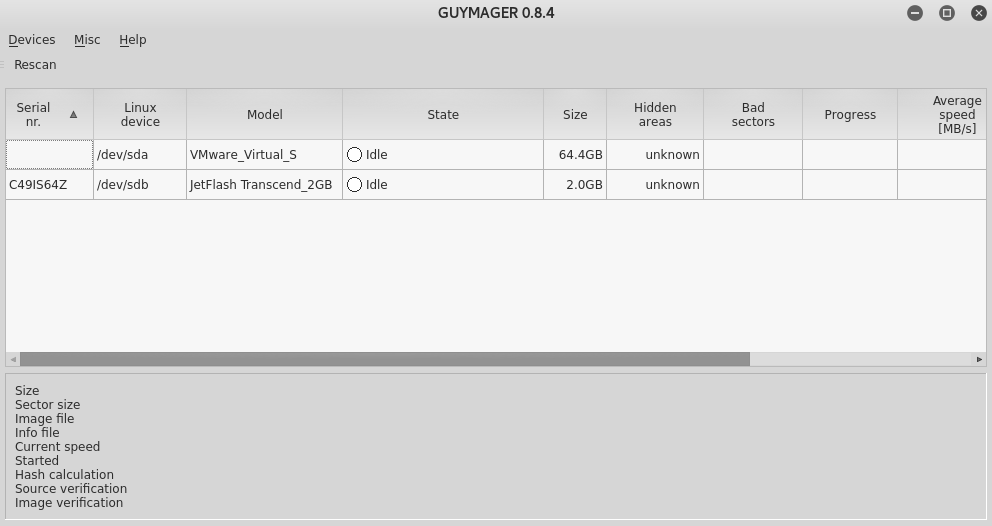
\includegraphics[scale=0.5]{guymager-window}
	\caption{\textit{guymager gui window example}}
	\label{fig:guymager-main-window}
\end{figure}
\\
If the 4GB USB drive does not show up press \texttt{f5} to rescan devices.  Select the drive you wish to create an image of in our case right click the 4GB drive and select the \texttt{acquire image} option. Fill out the displayed form making sure you have the following options selected as per the list below and/or \autoref{fig:guymager-aquisition-window} then click start:
\begin{itemize*}
\item Linux dd raw image
\item Uncheck split image
\item Destination is set to \texttt{/home/cases/001/image/}
\item Image filename set to \texttt{revmed2}
\item Info filename set to \texttt{revmed2}
\item Check calculate md5 hash
\item Check verify image after acquisition
\end{itemize*}
\begin{figure}[h]
	\centering
	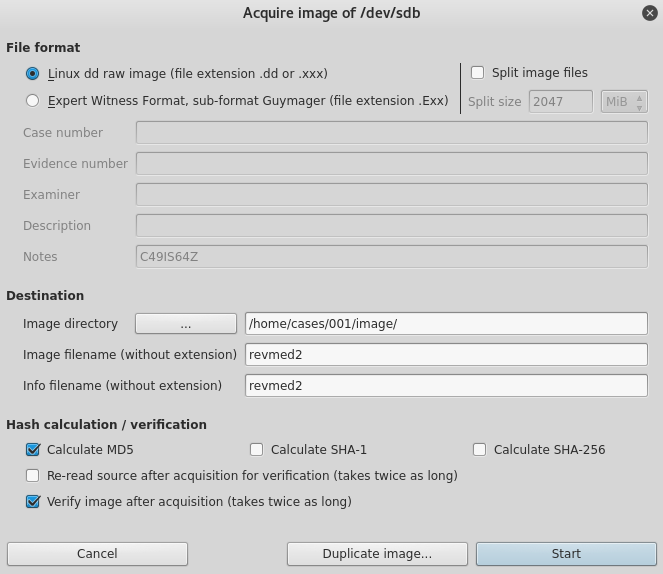
\includegraphics[scale=0.5]{guymager-aquisition-window}
	\caption{\textit{guymager acquisition window example}}
	\label{fig:guymager-aquisition-window}
\end{figure}

\newpage
Once you have clicked start you will be returned to the main \texttt{guymager} window and a progress bar should be displayed. Once the progress bar states ``Finished - Verified {\&} ok'' your forensic image have been created. To confirm list the contents of \texttt{/home/cases/001/image/} in a terminal window, you should find the following files: 
\begin{itemize*}
\item \texttt{revmed2.dd} : the image file we can now perform analysis on.
\item \texttt{revmed2.info} : acquisition info such as cryptographic hash.
\end{itemize*}

\subsubsection*{Verify The Media Hash}
In order to confirm that our.dd image is the same as the contents of the USB, we must generate a hash of the .dd file and compare it to the hash listed in the .info file.
\\
In a terminal window run the following:\\ \\
\texttt{{\#} md5sum image/revmed2.dd}\\
The output should match the hash listed in the .info file you just created.\\

\noindent
Remove the USB from your machine and return it to the evidence box.

\subsection*{Get Your Flag:}
\noindent
\textit{\textbf{Optional:} Enter the hash into the \texttt{findflag} program to receive your first flag.}

\end{document}